 \section{Lineare Vektorräume} 
		  
		  	\subsection{Koordinatensystem}
		  	Ein Koordinatensystem ist festgelegt durch: \\
		  	\begin{tabular}{ll}
		  	$\bullet$ & Ursprung O \\
		  	$\bullet$ & Basis bestehend aus linear unabh. Basisvekoren \textcolor{blue}{$b_i$} \\
		  	\\
		  	\end{tabular}
		  	
		  	Ortsvektor: \quad Vektor $\vv{OP}$ = $\vec{p}$ = $x_1 \cdot \textcolor{blue}{\vec{b_1}} + x_2 \cdot \textcolor{blue}{\vec{b_2}}$ \\
		  	\\
		  	$x_1$ und $x_2$ sind Koordinaten des Punktes P bzw. \\
		  	Linearkombinationen der Basisvektoren \textcolor{blue}{$b_i$}
		  	
		  	
			\subsection{Vektorraum  $\langle A \rangle$}		  
			Menge aller Koordinaten (Linearkombinationen), welche durch die Vektoren $A = \vec{a_1}, ... , \vec{a_n}$ erreicht werden können. \\
			\\
			Durch bilden weiterer Linearkombinationen (Skalierungen) der \\			
			Vektoren $\vec{a_i}$ verlässt man den Vektorraum nicht.\\
			\\
			Auch Additionen / Subtaktionen von Vektoren des Vektorraums verlassen den Verktorraum nicht. \\
			
			\vfill\null
			\columnbreak
			
			
			
			
			\subsubsection{Dimension}
			Die Dimension $\dim \langle A \rangle$ des Vektorraums besteht aus der maximalen Anzahl linear unabhängiger Vektoren im Vektorraum. \\
			$\rightarrow$ Linear abhängige Vektoren ändern die Dimension nicht!	  	
		  	
	  	
		  	\subsection{Basis eines Vektorraums}
		  	Die Basis eines Vektorraus muss die folgenden Kriterien erfüllen: \\
		  	\begin{tabular}{ll}
		  	1. & Lineare Unabhängigkeit der Basisvektoren \textcolor{blue}{$b_i$}, damit \\  
		  	& Koordinaten \textcolor{orange}{$x_i$} eindeutig sind \\
		  	2. & Basisvektoren \textcolor{blue}{$\vec{b_i}$} müssen den ganzen Vektorraum aufspannen \\
		  	\\
		  	\end{tabular}
		  		
		  	$\vec{p} = \textcolor{orange}{x_1} \cdot \textcolor{blue}{\vec{b_1}} + \textcolor{orange}{x_2} \cdot \textcolor{blue}{\vec{b_2}} + \textcolor{orange}{x_3} \cdot \textcolor{blue}{\vec{b_3}}$  = \textcolor{blue}{B} \textcolor{orange}x = $\begin{pmatrix}
1 & 0 & 0 \\ 0 & 1 & 0 \\ 0 & 0 & 1 	\end{pmatrix} \begin{pmatrix}
x_1 \\ x_2 \\ x_3
\end{pmatrix}$ \\

\vspace{0.2cm}

$\vec{b_1}$, $\vec{b_2}$ und $\vec{b_3}$ sind im Beispiel die Standardbasisvektoren. Es können aber auch irgendwelche Vektoren einer anderen Basis sein.


		  	
			\subsection{Basistransformation}		  	
			Basismatrix B = $\lbrace \vec{b_1}, \vec{b_2}, \vec{b_3} \rbrace$ \qquad Basismatrix B' = $\lbrace \vec{b_1'}, \vec{b_2'}, \vec{b_3'} \rbrace$		\\
	
			Vektor $\vec{v}$ = $\xi B$ = $\xi' B'$ in Koordinatensystem $\xi$ und $\xi'$
 
			\subsubsection{Basistransformation allgemeiner Fall}
			Transformationsmatrix T mittels Gauss-Algorithmus finden: \\
			\begin{minipage}{0.6\linewidth}
			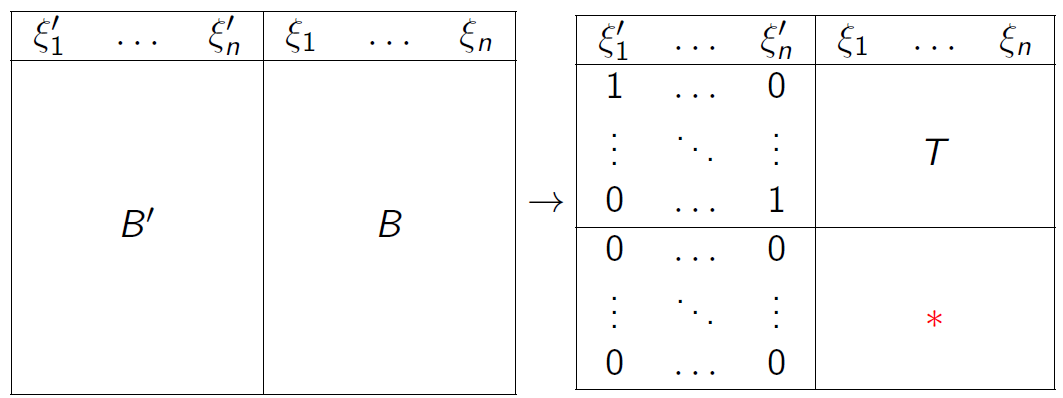
\includegraphics[width=\linewidth]{Bilder/transformationsmatrix} \\
			\end{minipage}
			\hfill
			\begin{minipage}{0.38\linewidth}
			$$ \text{Umrechnung:} \quad \xi' = T \xi$$
			\\
			\end{minipage}

			Die roten Sterne müssen Nullen sein, damit es eine Lösung gibt! 
			

			\subsubsection{Spezialfall Basistransformation (quadratische Matritzen)}		  
			\begin{tabular}{ll}
			Transfotmationsmatrix $T$ &  $T = (B')^{-1} B $	\\
			Koordinaten $\xi'$ in neuem Koordinatensystem: & $\xi = T \xi$ \\
			\end{tabular}				
				  	
		  	
		  	\subsection{Lineare Abbildungen (Bilder des Vektoraums)}
		  	\begin{tabular}{ll}
		  	Eine lineare Abbildung: & $\bullet$ bildet Geraden auf Geraden ab \\
		  	& $\bullet$ erhält Parallelität \\
		  	& $\bullet$ fixiert den Ursprung
		  	\end{tabular}
			
			Lineare Abbildungen werden mit der Abbildungsmatrix A \\
			beschrieben. \\		
			\textbf{Die Spalten von A sind Bilder der Basisvektoren} \\
			\\
			Eine Abbildung A kann durch ihre Inverse $A^{-1}$ rückgängig gemacht werden.
			
			
			
			
			\subsubsection{Beispiel Abbildungsmatrix A einer Scherung}
			Die Standardbasisvektoren $\vec{e_1}$ und $\vec{e_2}$ werden durch die Abbildungsmatrix $A$ auf die Vektoren $\vec{e_1'}$ und $\vec{e_2'}$ abgbildet. \\
			Die Spalten der Abbildungsmatrix A enthalten die Bilder $\vec{e_1'}$ und $\vec{e_2'}$ der Standardbasisvektoren 	$\vec{e_1}$ und $\vec{e_2}$ \\

			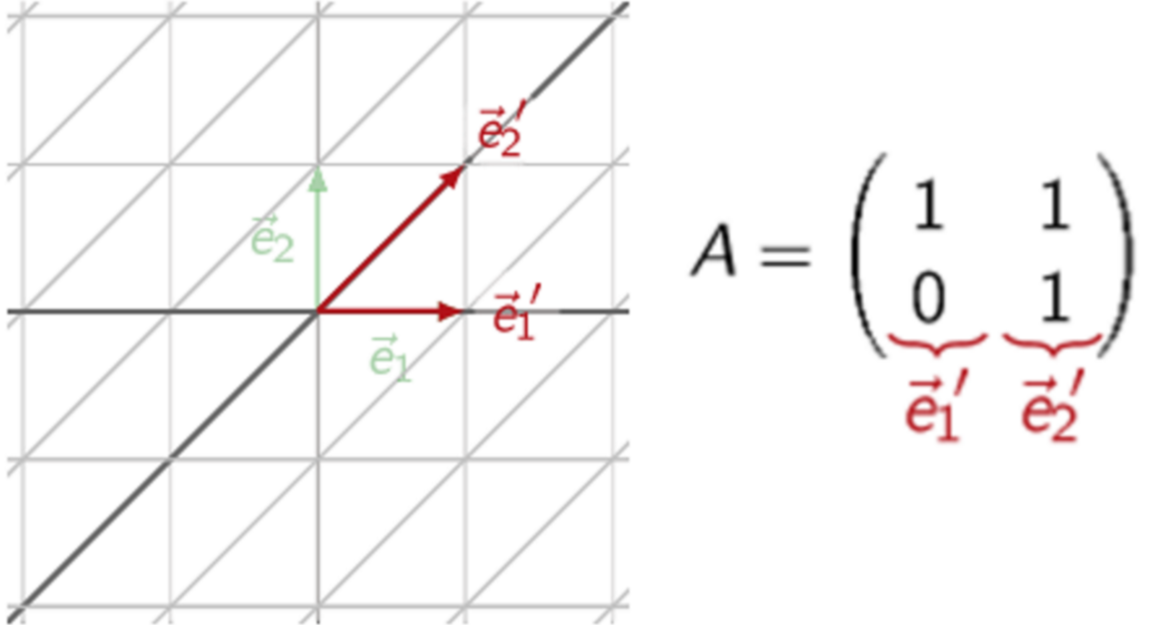
\includegraphics[width=0.5\linewidth]{Bilder/scherung}
			\subsubsection{Anwendung einer Abbildung auf einen Vektor}
			Der Vektor $\vec{v}$ wird mit der Abbildungsmatrix auf den Vektor $\vec{v'}$\\
			abgebildet: $A \cdot \vec{v} = \vec{v'}$ \\		
			\\		
			Die Abbildung kann mittels $A^{-1} \cdot \vec{v'} = \vec{v}$ rückgängig gemacht werden. \\
			\textbf{Das geht nur, wenn A eine quadratische Matrix ist!}

		  	\subsubsection{Zusammensetzung linearer Abbildungen}
		  	Wenn mehrere lineare Abbildungen "wirken", so werden die \\
		  	Abbildngsmatritzen multipliziert. \\
		  	\\
		  	\textbf{Die als erstes wirkende Abbildung steht dabei ganz rechts in der Multiplikation!}\\
		  	\\
		  	Abbildungsmatrix C = AB $\rightarrow$ Erst wirkt Abbildungsmatrix B,\\ 
		  	danach A
		  	
		  	
		  	\subsection{Kern einer Matrix}		
			Alle Abbildungen eines Vektors $\vec{v}$ , welche durch die \\
			Abbildungsmatrix $A$ auf den Nullvektor von $\vec{v'}$ abgebildet werden \\
			$A \cdot \vec{v} = 0 $ $\rightarrow$ Nullraum, Kern von $A$, ker($A$) 
			
			
			\subsection{Bild einer Matrix}		
			Menge der Vektoren, welche man aus den Spalten einer Matrix \\
			erzeugen kann.\\
			\\
			Das Bild besteht aus allen Vektoren, welche unter der Abbildung, die $B$ vermittelt, wentstehen können.
			
			
			\vfill\null
			\columnbreak
			
			
			
			\subsection{Kern, Bild und Gauss-Algorithmus}	
			Die Lösungsmenge entspricht dem Kern von $A$ bzw. dem Bild von $B$ \\	
			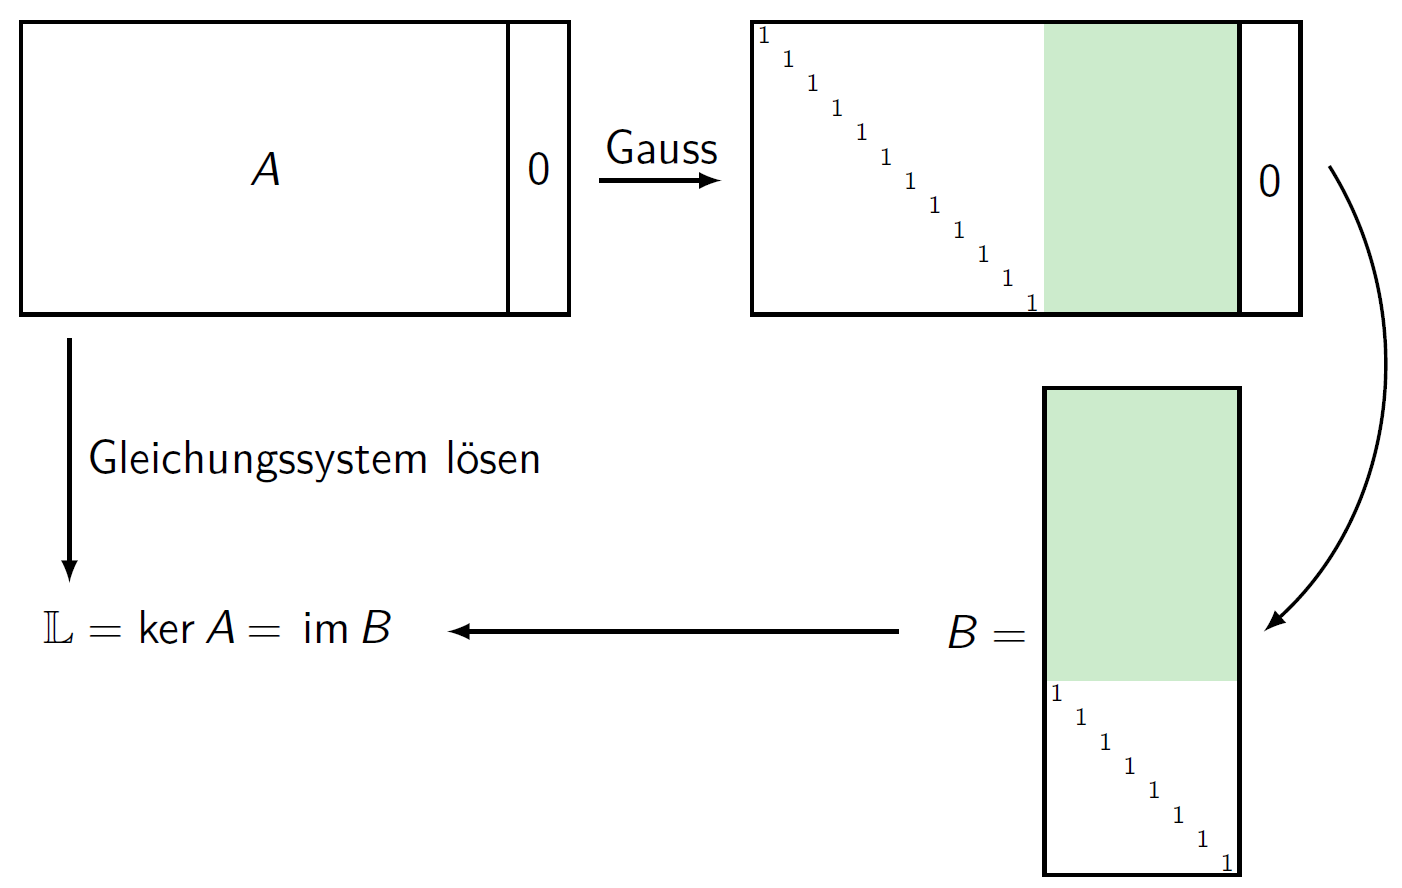
\includegraphics[width=0.55\linewidth]{Bilder/kern-bild-gauss} 	
			
			
			\subsection{Basiswechsel für lineare Abbildungen}
			Die lineare Abbildung, die in der Basis $B$ durch die Matrix $A$ beschrieben wird, wird in der Basis $C$ durch die Matrix $A'$ beschrieben.\\
			
			\begin{minipage}{0.6\linewidth}
			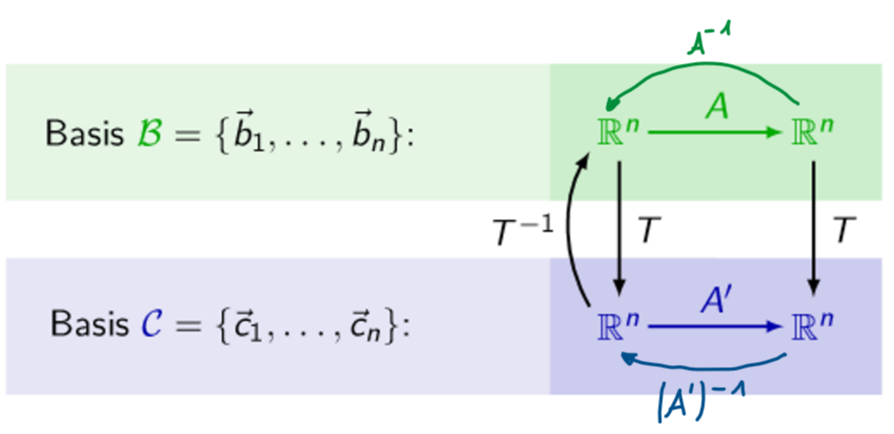
\includegraphics[width=0.9\linewidth]{Bilder/basiswechsel_abbildungen}
			\end{minipage}						
			\hfill
			\begin{minipage}{0.35\linewidth}
			$\textcolor{blue}{A'} = T \textcolor{green}A \,T^{-1}$ \\
			$\det(A') = \det(A)$ \\
			Spur($A'$) = Spur($A$)	
			\end{minipage}
	
		  	
		  	\subsection{Elementare Abbildungsmatritzten}
		  	\subsubsection{Drehmatrix D finden}
			Die Drehung wird beschrieben durch $D \cdot A = A'$		  	 \\
			Die Spalten der Matrix $A$ sind die Punkte vor der Drehung, $A'$ enthält die Punkte nach der Drehung (Bilder)\\
			$D = A' \cdot A^{-1}$ \\
			\textbf{Die Matritzten müssen quadratisch sein! Falls nötig Matritzen mit einem Punkt erweitern, damit sie quadratisch werden}
		  	
		  	
		  	\subsubsection{Spiegelungen (orthogonale Matrix)}
		  	$\det(A) = -1$ \\
		  	\\
		  	\textbf{2 Dimensionen} \\
		  	\\
		  	\begin{tabular}{lll}
		  	x-Achse & y-Achse & an 45° Geraden \\
		  	\\
		  	$\begin{pmatrix} 1 & 0 \\ 0 & -1 \end{pmatrix}$ & $\begin{pmatrix} -1 & 0 \\ 0 & 1 \end{pmatrix}$ & $\begin{pmatrix} 0 & 1 \\ 1 & 0 \end{pmatrix}$ \\
		  	\\
		  	\end{tabular}
		  	
			\textbf{3 Dimensionen} \\
		  	\\
		  	\begin{tabular}{lll}
		  	xy-Ebene & xz-Ebene & an yz-Ebene\\
		  	\\
		  	$\begin{pmatrix} 1 & 0 & 0 \\ 0 & 1 & 0 \\ 0 & 0 & -1 \end{pmatrix}$ & $\begin{pmatrix} 1 & 0 & 0 \\ 0 & -1 & 0 \\ 0 & 0 & 1 \end{pmatrix}$ & $\begin{pmatrix} -1 & 0 & 0 \\ 0 & 1 & 0 \\ 0 & 0 & 1 \end{pmatrix}$ \\
		  	\end{tabular}		  	
		  	
			\subsubsection{Projektionen}		
			Projektionen auf etwas (z.B. die Koordinatenachsen) liefern die "Länge des Schattens" des Vektors auf diese Achse. \qquad $P^2 = P$ \\
			\\
			\begin{tabular}{ll}
		  	x-Achse & y-Achse \\
		  	\\
		  	$\begin{pmatrix} 1 & 0  \\ 0 & 0  \end{pmatrix}$ & $\begin{pmatrix} 0 & 0  \\ 1 & 0  \end{pmatrix}$  \\
		  	\\
		  	\end{tabular}				
			
			\begin{tabular}{lll}
		  	xy-Ebene & xz-Ebene & an yz-Ebene\\
		  	\\
		  	$\begin{pmatrix} 1 & 0 & 0 \\ 0 & 1 & 0 \\ 0 & 0 & 0 \end{pmatrix}$ & $\begin{pmatrix} 1 & 0 & 0 \\ 0 & 0 & 0 \\ 0 & 0 & 1 \end{pmatrix}$ & $\begin{pmatrix} 0 & 0 & 0 \\ 0 & 1 & 0 \\ 0 & 0 & 1 \end{pmatrix}$ \\
		  	\end{tabular}		  	
		  	
		  	\subsubsection{Drehungen D (orthogonale Matrix)}
		  	Die Spalten von $D_{\alpha}$ sind Bilder der Basisvektoren \\
		  	Determinante: \quad $\det(D) = 1$\\	
		  	\\
		  	Die Drehung findet gegen den Uhrzeigersinn statt \\
		  	Für Drehung in Uhrzeigersinn: $D_{-\alpha} = D_{\alpha}^{-1}$ verwenden \\
		  	$D_{\alpha} D_{\beta} = D_{\alpha + \beta}$ \\
		  	\\		  	
		  	\textbf{2 Dimensionen} \\
		  	\\
		  	$D_{\alpha} = \begin{pmatrix} \cos(\alpha) & -\sin(\alpha)  \\ \sin(\alpha) & \cos(\alpha)  \end{pmatrix}$ \\
		  	
			\textbf{3 Dimensionen} \\
			\\
			\begin{tabular}{ll}
			Drehung um x-Achse & Drehung um y-Achse \\
			\\
			$D_{x} = \begin{pmatrix} 1 & 0 & 0 \\\
			0 & \cos(\alpha) & -\sin(\alpha)  \\ 0 & \sin(\alpha) & \cos(\alpha)  \end{pmatrix}$ & $D_{y} = \begin{pmatrix} \cos(\alpha) & 0 & \sin(\alpha) \\
			0 & 1 & 0 \\ -\sin(\alpha) & 0 & \cos(\alpha)  \end{pmatrix}$\\
			\\
			Drehung um z-Achse & \\
			\\
			$D_{z} = \begin{pmatrix} \cos(\alpha) & -\sin(\alpha) & 0 \\ \sin(\alpha) & \cos(\alpha) & 0 \\ 0 & 0 & 1 \end{pmatrix}$
			\end{tabular}
		  	
		  	
			\subsection{Drehwinkel von Drehmatritzen D}		  	
			Der Drehwinkel einer Drehmatrix $D$ wird mithilfe der Spur der \\
			Drehmatrix berechnet (siehe nächster Abschnitt) \\ 	
			\\	  			
			\begin{tabular}{lll}
			\textbf{2 Dimensionen} & & \textbf{3 Dimensionen} \\
			\\
			$\cos(\alpha) = \frac{\mathrm{Spur}(D)}{2}$ & & $\cos(\alpha) = \frac{\mathrm{Spur}(D) -1}{2}$
			\end{tabular}
		  	
			\vfill\null
			\columnbreak		  	
		  	
		  	
			\subsection{Spur}		  	
			Die Spur einer Matrix ist die Summe der Elemente auf der Diagonalen \\
			
			$A =  \begin{pmatrix}	\textcolor{blue}{1} & 7 & 9 \\ 2 & \textcolor{blue}{9} & 6 \\ 8 & 3 & \textcolor{blue}{5}	\end{pmatrix}$	   \qquad 	$\mathrm{Spur}(A) = \textcolor{blue}{1} + \textcolor{blue}{9} + \textcolor{blue}{5} = 15$ 
		  	
		  	\subsubsection{Rechenregeln Spur}
		  	\begin{tabular}{ll}
		  	Vertauschung & Spur($BA$) = Spur($AB$) \\
		  	Zykl. Vertauschung: & Spur($ABC$) = Spur($CAB$) = Spur($BCA$)\\
		  	Anwendung: & Spur($TAT^{-1}$) = Spur($T^{-1}TA$)= Spur($A$)\\
		  	\end{tabular}
		  	